% Section and frames
\section{DATA OVERVIEW}
\label{data_overview_section}

% Section title slide
\sectiontitleframe{DATA OVERVIEW}

% Slide 1: Dataset Description
\begin{frame}{Dataset Description}
    \frametitle{Exploring the Dataset}
    \begin{itemize}
        \item Created by Dean De Cock for educational purposes.
        \item Already splitted into training and test set.
        \item 79 quantitative and categorical variables.
        \item Feature examples: 'LotArea', 'YearBuilt', 'KitchenQual', etc.
    \end{itemize}
    \vspace{0.5cm}
    \begin{figure}
        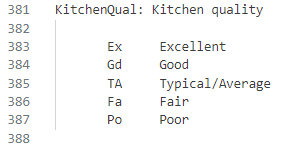
\includegraphics[width=0.4\textwidth]{figures/data_description.png} 
        \caption{Dataset Description Snapshot.}
        \label{fig:dataset_description_snapshot}
    \end{figure}
\end{frame}

% Slide 2-4: Dataset Samples and Statistics
\begin{frame}{Dataset Samples}
    \frametitle{Sample Data Overview}
    \begin{figure}
        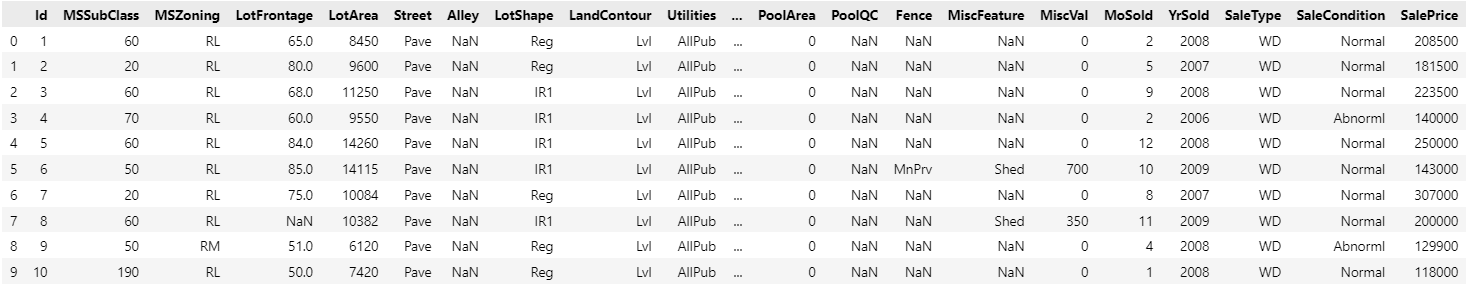
\includegraphics[width=1\textwidth]{figures/data_head.png} 
        \caption{Information of ten samples.}
        \label{fig:dataset_head}
    \end{figure}
\end{frame}

\begin{frame}{Dataset Statistics - Numerical}
    \frametitle{Statistical Insights}
    \begin{itemize}
        \item Numerical summary of the dataset (mean, median, mode, etc.).
        \item Include tables or bullet points with key statistics.
    \end{itemize}
\end{frame}

\begin{frame}{Dataset Statistics - Visualisation}
    \frametitle{Visual Statistical Analysis}
    \begin{itemize}
        \item Visualisation of dataset statistics (histograms, box plots, etc.).
        \item Insights derived from visual analysis.
    \end{itemize}
\end{frame}

% Slide 5-7: Data Engineering Methods
\begin{frame}{Data Engineering Methods}
    \frametitle{Data Preprocessing Techniques}
    \begin{itemize}
        \item Overview of data engineering techniques used.
        \item Methods: Missing value handling, data cleaning, integration.
        \item Data standardization (normalization) and transformation processes.
        \item Visuals or examples of these processes (to be added).
    \end{itemize}
\end{frame}

% Example frame 1
% \begin{frame}{frame} % set section name
%     \frametitle{frame}
%     \begin{itemize}
%         % Dataset Description
%         \item 1-2 slides
%         \item Describe the dataset (purpose, contents overview, creator, number of features, names of features…)
%         % Dataset Statistics
%         \item 3-5 slides
%         \item Present first couple of samples in the dataset
%         \item Present the statistics of the dataset, using both numerical and visualisation methods (please refer to the homework tasks)
%         % Data Engineering
%         \item 1-3 slides
%         \item Present what methods of data engineering you used in your work here (Missing values, Data cleaning, Data integration, Data standardization (normalization), Data transformation…)
%         \item Describe the reason and for using those methods
%         \item Present the effect of applying these methods
%     \end{itemize}
% \end{frame}